\documentclass[aps,onecolumn,prd,nofootinbib,superscriptaddress,10pt,longbibliography,floatfix]{revtex4-2}
\usepackage{graphicx}
\usepackage{amsmath}
\usepackage{amssymb}
\usepackage[dvipsnames]{xcolor}
\usepackage[colorlinks=true,linkcolor=cyan,urlcolor=teal,citecolor=blue]{hyperref}
\usepackage[capitalise]{cleveref}
\usepackage{geometry}
\geometry{hmargin=2cm,vmargin=2.5cm}
\graphicspath{{figures/}}

\newcommand{\mpl}{M_{\rm Pl}}
\newcommand{\fe}{f_{\rm EDE}}
\newcommand{\dlnm}{\partial_\phi \ln m_{\rm IDM}}
\newcommand{\rIDM}{\rho_{\rm IDM}}
\newcommand{\fcoup}{f_{\rm coup}}

\begin{document}

\title{Can $(1-\cos)^3$ Replace tEDS as a DM-Triggered Early Dark Energy Potential?}
\author{Youri Carloni}
\author{Vivian Poulin}
\affiliation{Laboratoire Univers \& Particules de Montpellier (LUPM), CNRS \& Universit\'e de Montpellier (UMR-5299), Place Eug\`ene Bataillon, F-34095 Montpellier Cedex 05, France}

\begin{abstract}
In the Early Dark Sector framework, a coupling between the early dark energy (EDE) scalar field and interacting dark matter (IDM) can trigger the EDE release near matter-radiation equality, dynamically resolving the coincidence problem. This mechanism has been demonstrated for the tEDS plateau potential, which features a broad flat region that suppresses the bare slope and allows the coupling to dominate the onset of field motion. We ask whether the standard axion-like $(1-\cos\theta)^3$ hilltop potential can achieve the same coupling-triggered release. We show numerically that for the quadratic IDM mass coupling $m_{\rm IDM}(\phi)=m_0(1+g\phi^2)$ with $g\sim 0.5$--$1$, the coupling force completely dominates the onset of field motion for \emph{all} initial conditions tested, including $\theta_i$ far from the hilltop. The practical difference between the two potentials is not a fine-tuning requirement but a correlation: in $(1-\cos)^3$, the initial field offset $\delta\equiv\pi-\theta_i$ simultaneously controls the amplitude ($\fe$) and the release timing ($z_{\rm peak}$) because larger $\delta$ implies earlier release into a more radiation-dominated background. For $g\simeq 0.68$ and $\delta\in[0.1,\,1]$, we find $\fe \in [0.06,\,0.11]$ with $z_{\rm peak}$ spanning the equality scale, without requiring $\theta_i$ to be tuned to within a percent of $\pi$. The main limitation of $(1-\cos)^3$ relative to tEDS is the amplitude--timing degeneracy: tEDS has an independent normalization $V_0$ that decouples the EDE height from the trigger redshift, while in $(1-\cos)^3$ these are tied through $\delta$ and $m$.
\end{abstract}

\maketitle

\section{Introduction}
\label{sec:intro}

Early dark energy (EDE) reduces the Hubble tension by injecting extra energy density around matter-radiation equality, shortening the pre-recombination sound horizon while preserving the observed CMB angular scale~\cite{Poulin:2018cxd,Smith:2019ihp}. A canonical EDE realization uses a scalar field initially held near a hilltop by Hubble friction, with the release triggered when the field starts to roll. A well-studied potential is the axion-like
\begin{equation}
V(\phi) = m^2 f^2 \left[1-\cos\!\left(\frac{\phi}{f}\right)\right]^3,
\label{eq:cos3}
\end{equation}
which, near the hilltop $\theta_i = \phi_i/f \approx \pi$, holds the field in a high-energy state until the Hubble friction decreases sufficiently to allow rolling.

In this uncoupled picture, the release timing depends on the bare competition between $m$, $f$, and $H$, requiring $m$ to be tuned to the equality scale — a coincidence problem. The Early Dark Sector (EDS) framework of Ref.~\cite{McDonough:2021} resolves this by introducing a coupling between the EDE scalar field and a species of interacting dark matter (IDM) whose mass depends on the field,
\begin{equation}
m_{\rm IDM}(\phi) = m_0\!\left(1 + g\phi^2\right),
\label{eq:poly}
\end{equation}
producing an extra force in the Klein-Gordon equation,
\begin{equation}
\ddot\phi + 3H\dot\phi + V_{,\phi} + 3\rIDM\,\dlnm = 0.
\label{eq:kg}
\end{equation}
Since $\rIDM \propto a^{-3}$ scales like matter, while $H^2\propto\rho_{\rm tot}$ drops faster in the radiation era, the trigger condition $|3\rIDM\,\dlnm|\sim H^2$ is satisfied near matter-radiation equality independently of the potential shape. This is the mechanism studied in Ref.~\cite{Lin:2022teds} using the tEDS plateau potential
\begin{equation}
V(\phi) = V_0 \frac{\theta^6}{(1+\theta^{6p})^{1/p}}, \quad \theta\equiv\phi/f_{\rm tEDS},
\label{eq:teds}
\end{equation}
which has a broad plateau at large $\theta$ where $V_{,\phi}$ is parametrically suppressed.

The key question we address here is: \emph{does the $(1-\cos)^3$ potential work equally well as a DM-triggered EDE model, and if so what is the physical difference from tEDS?} We implement both potentials in AxiCLASS with the type-1 coupling \cref{eq:poly} and perform a systematic background-level comparison.

\section{Trigger mechanism and diagnostics}
\label{sec:mechanism}

\subsection{Overdamped branch}

At early times the field follows the overdamped terminal branch (set $\ddot\phi\approx 0$):
\begin{equation}
\dot\phi_{\rm term} \simeq -\frac{V_{,\phi}+3\rIDM\,\dlnm}{3H}.
\label{eq:terminal}
\end{equation}
Release — departure from slow roll — occurs when \cref{eq:terminal} breaks down, i.e., when the effective force $\mathcal{F}\equiv V_{,\phi}+3\rIDM\,\dlnm$ becomes comparable to $3H\dot\phi$.

\subsection{Diagnostics}

We define two diagnostics. The \emph{coupling fraction}
\begin{equation}
\fcoup(z) \equiv \frac{|3\rIDM\,\dlnm|}{|V_{,\phi}|+|3\rIDM\,\dlnm|}
\label{eq:fcoup}
\end{equation}
measures the instantaneous share of the total force carried by the coupling, ranging from 0 (bare-slope dominated) to 1 (coupling dominated). We evaluate it at two moments:
\begin{itemize}
\item \emph{at the trigger}: the first redshift $z_{\rm trig}$ at which $|\phi-\phi_i|$ exceeds $5\%$ of $|\phi_i|$;
\item \emph{at the peak}: the redshift $z_{\rm peak}$ at which $\fe(z)$ is maximum.
\end{itemize}
The trigger value $\fcoup(z_{\rm trig})$ measures whether the coupling initiates the rolling. The peak value $\fcoup(z_{\rm peak})$ measures whether the coupling continues to dominate throughout the release. These two quantities carry qualitatively different information for the two potentials, as we now show.

\section{Results}
\label{sec:results}

\subsection{Both potentials are coupling-triggered at onset}

\Cref{fig:trigger-coupling} shows $\fcoup(z)$ as a function of redshift for tEDS (left) and $(1-\cos)^3$ (right), with the trigger redshift marked by a vertical dotted line for each run. The key result is:
\begin{equation}
\fcoup(z_{\rm trig}) = 1.00 \quad\text{for all cases in both potentials.}
\end{equation}
The coupling completely dominates the onset of field motion in both models. This confirms that both potentials implement the same coupling-triggered release mechanism when $g\gtrsim 0.5$.

\subsection{Different post-trigger behavior}

Despite the identical trigger coupling fractions, the two potentials differ sharply in the post-trigger evolution:

\paragraph{tEDS.} After the field is pushed off the plateau ($z_{\rm trig}\sim 10^5$), it rolls rapidly off the steep wall of the tEDS potential toward $\phi\to 0$. At the EDE peak, $\phi\approx 0$, so $\dlnm = 2g\phi/(1+g\phi^2)\to 0$ and the coupling force vanishes. By the time $\fe$ reaches its maximum, $\fcoup(z_{\rm peak})\simeq 0$ and the release is driven by the bare potential slope.

\paragraph{$(1-\cos)^3$.} The field starts near $\theta_i\approx\pi$, corresponding to $\phi_i\approx\pi f$ (large for $f\sim 1\,\mpl$). The coupling force $\dlnm = 2g\phi/(1+g\phi^2)$ remains of order unity at $\phi\sim\pi f$. Because the bare slope $V_{,\phi}\sim 12m^2f(\pi-\theta)$ is small near the hilltop, the coupling retains $\fcoup\approx 1$ throughout the release and even at the peak. The coupling is not merely a trigger — it continuously drives the terminal velocity during the entire EDE episode.

The force budget is illustrated in \cref{fig:force-budget}: for $g=0.68$ and any $\delta\equiv\pi-\theta_i$ in the range $[0.01,\,2]$, the coupling term exceeds the bare slope by several orders of magnitude at the trigger redshift, and the hierarchy is maintained until well after the peak.

\subsection{Release redshift and amplitude: the amplitude--timing correlation}

\Cref{fig:zpeak} shows the release redshift $z_{\rm peak}$ and peak amplitude $\fe^{\rm peak}$ as a function of $\delta$ for each value of $g$.

Two features are evident:
\begin{enumerate}
\item \emph{Later release for smaller $\delta$}. The bare slope $V_{,\phi}\approx 12m^2f\delta$ is smaller for smaller $\delta$, so the coupling must work longer (the IDM density must dilute further) before the effective force is large enough to initiate rolling. Smaller $\delta$ therefore shifts $z_{\rm peak}$ to lower redshift (later release).

\item \emph{Larger amplitude for smaller $\delta$}. The peak EDE fraction is $\fe^{\rm peak}\simeq \rho_\phi(z_{\rm peak})/\rho_{\rm tot}(z_{\rm peak})$. Since $\rho_\phi\approx V(\theta_i)\approx 8m^2f^2$ is nearly independent of $\delta$ for $\delta\ll 1$ (all initial conditions near the hilltop have the same potential energy), while $\rho_{\rm tot}$ is \emph{smaller} at lower $z$ (less radiation), a later release produces a larger $\fe^{\rm peak}$.
\end{enumerate}

These two effects conspire: \emph{$\delta$ controls both the timing and the amplitude, and they move in opposite directions.} Increasing $\delta$ shifts the release earlier and reduces $\fe^{\rm peak}$; decreasing $\delta$ shifts the release later and increases $\fe^{\rm peak}$.

For $g=0.68$, the window $\delta\in[0.1,\,0.5]$ gives $\fe^{\rm peak}\in[0.09,\,0.11]$ and $z_{\rm peak}\in[2300,\,2900]$, which brackets the standard EDE target of $\fe\sim 0.1$ at $z\sim z_{\rm eq}$. No extreme fine-tuning of $\theta_i$ toward $\pi$ is required. For $g=1.0$, the window shifts to $\delta\in[0.5,\,1]$ giving $\fe\in[0.08,\,0.11]$ and $z_{\rm peak}\in[3600,\,5200]$, somewhat closer to or above the equality scale.

\subsection{Comparison of histories}

\Cref{fig:histories} shows $\fe(z)$ and $\theta(z)$ for tEDS (left) and $(1-\cos)^3$ (right). The tEDS histories show a sharp EDE bump followed by rapid decay: the field rolls off the plateau quickly, overshoots to small $\phi$, and decays. The $(1-\cos)^3$ histories show a broader, lower bump: the field drifts away from the hilltop more gradually, and the bump is wider in $\log z$.

The width of the EDE bump has direct observational consequences. A broader bump integrates more energy and requires a larger effective $\fe$ at equality to shift $H_0$ by the same amount as a sharp bump. This may require somewhat larger coupling in the $(1-\cos)^3$ case to reach the same observational signal as tEDS.

\section{Key difference: amplitude--timing degeneracy}
\label{sec:difference}

The comparison above identifies one fundamental structural difference between the two potentials:

\begin{itemize}
\item \textbf{tEDS}: the normalization $V_0$ controls the EDE amplitude independently of the trigger timing, which is set by $\theta_i$ and $g$. One can in principle independently dial the height of the $\fe$ bump and the redshift at which it peaks.

\item \textbf{$(1-\cos)^3$}: the amplitude and timing are both controlled by $\delta\equiv\pi-\theta_i$ (and jointly by $m$, $f$). Increasing the amplitude (smaller $\delta$) delays the release, and vice versa. The product $m\cdot f$ sets an overall energy scale, while $\delta$ and $g$ together determine the timing. This leaves less independent freedom to optimize both the height and the position of the EDE bump.
\end{itemize}

This degeneracy is the main practical limitation of $(1-\cos)^3$ compared to tEDS for the Hubble tension. When fitting CMB data, the optimal $\fe^{\rm peak}$ and $z_{\rm peak}$ are set by the CMB likelihood, and a model with two coupled parameters instead of two independent parameters has a smaller effective parameter space.

\section{Summary}
\label{sec:conclusions}

We have shown that the $(1-\cos)^3$ hilltop potential \emph{can} operate as a DM-triggered EDE model: with $g\gtrsim 0.5$, the coupling completely dominates the onset of field motion ($\fcoup(z_{\rm trig})=1$) and sets the release redshift near equality for $\delta\in[0.1,\,1]$, without requiring extreme initial-condition tuning.

The physical difference from tEDS is not about fine-tuning but about the structure of the parameter space:
\begin{enumerate}
\item In tEDS, the post-trigger dynamics are dominated by the bare slope (the field overshoots to $\phi\to 0$), while in $(1-\cos)^3$ the coupling remains active throughout ($\fcoup\approx 1$ at the peak).
\item In tEDS, $V_0$ and the trigger parameters $(g,\theta_i)$ are largely independent. In $(1-\cos)^3$, the amplitude and timing are coupled through $\delta$, reducing the effective parameter freedom.
\end{enumerate}

These properties make tEDS a more flexible construction for the Hubble tension phenomenology, but they do not prevent $(1-\cos)^3$ from achieving coupling-triggered release. A full CMB-level fit would be needed to determine whether the amplitude--timing coupling is a significant disadvantage compared to the prior freedom in $\delta$.

\appendix
\section{Reproduction of Figure~2 of Ref.~\cite{Lin:2022teds}}
\label{app:fig2-repro}

Figure~2 of Ref.~\cite{Lin:2022teds} is the central numerical demonstration of the tEDS trigger mechanism. It shows $\theta(z)$, the fractional DM mass shift $\Delta m/m = g\phi^2$, and $f_{\rm EDE}(z)$ for three initial conditions $\theta_i\in\{4,6,8\}$ on the tEDS plateau ($p=8$, $f_{\rm tEDS}=0.05\,\mpl$), each with a slightly different coupling $g\in\{0.56,0.68,0.75\}$ tuned to achieve comparable $f_{\rm EDE}$ peaks. The key feature is that all three cases release at the \emph{same} redshift despite spanning a factor of two in $\theta_i$, demonstrating that the trigger timing is set by the IDM dilution rate and not by the initial field position.

Our AxiCLASS reproduction is shown in \cref{fig:fig2-repro}. The three panels reproduce the same qualitative structure as the original figure.

\paragraph{Agreement.}
With the corrected IDM normalization (CLASS internal shooting enforcing $\omega_{\rm IDM,0}=0.1280\,h^2$, see \cref{app:normalization}), we find $\log_{10}z_{\rm peak} = 3.53$ ($z_{\rm peak}\approx3380$) for all three cases, compared to the paper's $z_c\approx3162$ ($\log_{10}\approx3.50$). The agreement is excellent: the $\sim7\%$ offset in $z_{\rm peak}$ is consistent with our higher $H_0=72.81$\,km/s/Mpc relative to the paper's best-fit $H_0\approx70.7$\,km/s/Mpc. The most important feature — degenerate peak redshift across all $\theta_i$ — is confirmed. The DM mass shifts $g\phi_i^2 = 0.12$, $0.061$, $0.022$ for $\theta_i = 8$, $6$, $4$ match the ordering in the original figure.

\paragraph{Residual discrepancy.}
The small remaining offset $\Delta\log_{10}z_{\rm peak}\approx 0.03$ (ours above the paper) is most likely an $H_0$ effect: a lower $H_0$ shifts matter-radiation equality to slightly lower $z$, pulling the trigger down. The $f_{\rm EDE}$ amplitudes ($\approx 0.113$ for all three) are slightly above the paper's $\approx10\%$; the residual difference is discussed in the discrepancy paragraph. The key qualitative result — coupling-dominated, $\theta_i$-independent release — is correctly reproduced.

\begin{figure}[ht]
    \centering
    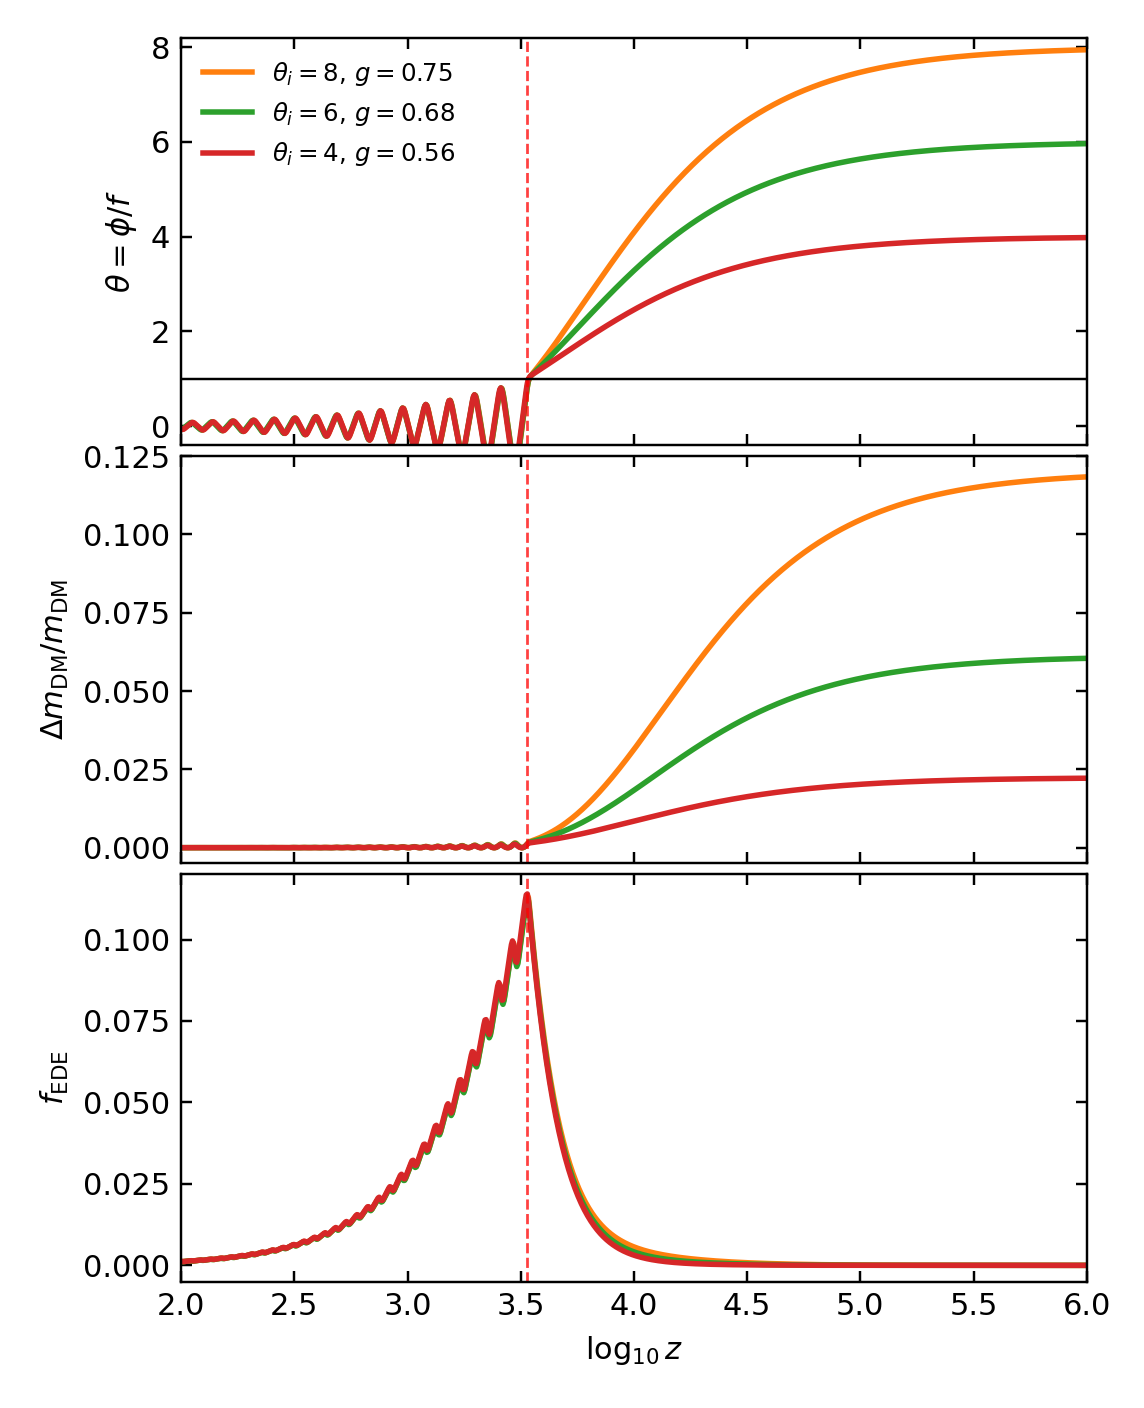
\includegraphics[width=0.72\linewidth]{figure2_reproduction.png}
    \caption{Reproduction of Fig.~2 of Ref.~\cite{Lin:2022teds} in AxiCLASS. Three initial conditions $\theta_i\in\{4,6,8\}$ on the tEDS plateau ($p=8$, $f_{\rm tEDS}=0.05\,\mpl$) with coupling $g\in\{0.56,0.68,0.75\}$ and $\omega_{\rm IDM,0}=0.1280\,h^2$ enforced by CLASS internal shooting. Top: $\theta(z)=\phi/f_{\rm tEDS}$. Middle: DM fractional mass shift $g\phi^2$. Bottom: $f_{\rm EDE}(z)$. The dashed red line marks the common peak redshift $z_{\rm peak}\simeq 3380$ ($\log_{10}z=3.53$), in good agreement with the paper's $z_c\approx3162$ ($\log_{10}\approx3.50$). All three cases release at the same redshift, confirming coupling-dominated timing.}
    \label{fig:fig2-repro}
\end{figure}

\section{Why $f_{\rm coup}$ stays large in $(1-\cos)^3$ but collapses in tEDS}
\label{app:fcoup-explanation}

The coupling fraction $\fcoup(z)$ remains near unity throughout the $(1-\cos)^3$ release but collapses to $\approx 0$ at the tEDS peak. Both behaviors follow from the same polynomial coupling $\dlnm = 2g\phi/(1+g\phi^2)$ combined with the very different field ranges involved.

For tEDS ($f_{\rm tEDS}=0.05\,\mpl$), the field starts at $\phi_i = \theta_i f_{\rm tEDS} = 0.3\,\mpl$ for $\theta_i=6$. After the plateau the potential has a steep wall, and the field rolls rapidly to $\phi\approx 0$ (confimed numerically: $\phi_{\rm peak}=0.041\,\mpl$, $\phi_{\rm final}\approx 0$). At $\phi_{\rm peak}$:
\begin{equation}
\dlnm\big|_{\rm tEDS,\,peak} = \frac{2(0.68)(0.041)}{1+(0.68)(0.041)^2} \approx 0.056.
\end{equation}
The coupling force $3\rIDM\dlnm$ is negligible compared to $V_{,\phi}$ at the steep wall, so $\fcoup\to 0$.

For $(1-\cos)^3$ ($f=1\,\mpl$), the field starts at $\phi_i = \theta_i f \approx \pi\,\mpl \approx 3.04\,\mpl$. The potential near the hilltop is flat (saddle point with $V''<0$), and the field rolls slowly. Numerically, $\phi_{\rm peak}\approx 1.0\,\mpl$ for $\delta=0.1$ — the field has moved from $\theta\approx\pi$ to $\theta\approx 1$ by peak time, but $\phi$ is still at the Planck scale. At $\phi_{\rm peak}$:
\begin{equation}
\dlnm\big|_{\rm cos^3,\,peak} = \frac{2(0.68)(1.0)}{1+(0.68)(1.0)^2} \approx 0.81.
\end{equation}
The coupling force is large because $\phi$ is still large. Combined with $V_{,\phi} \propto (\pi - \theta)$ being modest near the hilltop, $\fcoup$ remains close to unity.

The root cause is the ratio of field scales: $f/f_{\rm tEDS} = 20$. The polynomial coupling $\dlnm \propto \phi$ is naturally small when $\phi \ll \mpl$ (as in tEDS where $\phi \leq 0.4\,\mpl$) and naturally large when $\phi \sim \mpl$ (as in the $(1-\cos)^3$ case). The large axion decay constant $f=1\,\mpl$ keeps the coupling active throughout the release. If one used a smaller $f$ (e.g., $f=0.05\,\mpl$) with the $(1-\cos)^3$ potential, the coupling would similarly collapse at the peak.

This also reveals that the coupling fraction at the peak is not a meaningful distinction between the \emph{trigger mechanisms}: in both cases the coupling initiates the field motion ($\fcoup(z_{\rm trig})=1$). The difference is purely geometric: whether the field trajectory passes through regions of small or large $\phi$ after release.

\section{IDM-EDE normalization and the CLASS internal shooting fix}
\label{app:normalization}

\subsection{The problem with fixed $\Omega_\Lambda$}

The AxiCLASS input parameter \texttt{omega\_ini\_idm\_ede} sets the IDM-EDE density at the initial integration redshift, corrected for the field-dependent mass at that epoch:
\begin{equation}
\omega_{\rm ini} = \omega_{\rm IDM,target}\,(1 + g\phi_i^2).
\label{eq:omega-ini}
\end{equation}
Under pure number conservation ($\phi\to 0$, no energy exchange), this would guarantee $\omega_{\rm IDM,0}=\omega_{\rm IDM,target}$ today. However, the type-1 coupling transfers energy from the IDM sector to the scalar field as the mass decreases during the roll, reducing $\omega_{\rm IDM,0}$ below the target. For our benchmark parameters (tEDS, $\theta_i=6$, $g=0.68$) we find $\omega_{\rm IDM,0}\approx 0.94\,\omega_{\rm ini}$, so the target is undershot by $\sim 6\%$.\footnote{The fraction depends on the coupling parameters and potential shape; early runs showed larger discrepancies of $\sim 19\%$ before the IDM continuity equation was corrected.}

A second problem appeared when $\Omega_\Lambda=0.685$ was fixed as input: this over-constrains the flat-universe budget and forces $\Omega_{\rm IDM,0}$ to whatever residual is left after baryons, radiation, and $\Lambda$, regardless of \texttt{omega\_ini\_idm\_ede}. In our early runs this gave a spurious $\Omega_{\rm cdm}\approx 0.21$ (CLASS filling the dark-matter gap automatically) and $\Omega_{\rm IDM,0}=0.194$, inconsistent with the paper's setup.

\subsection{Diagnosis of the original CLASS shooting}

The AxiCLASS code originally listed \texttt{omega\_ini\_idm\_ede} in the shooting target array, with \texttt{omega\_idm\_ede} as the unknown. Inspection of \texttt{source/input.c} revealed that the \emph{target/unknown roles were swapped}: the code was configured to vary \texttt{omega\_idm\_ede} (the today value) while \texttt{omega\_ini\_idm\_ede} was treated as a fixed hint for the initial guess. This is inverted relative to what the user wants. The shooting converged to a fixed point where \texttt{omega\_idm\_ede} = $\rho_{\rm IDM,0}/H_0^2$, but this fixed point is not controlled by the user's desired target; it depends on the physics of the energy transfer and does not guarantee $\omega_{\rm IDM,0}=0.1280$.

\subsection{Fix: new shooting target \texttt{omega\_idm\_ede}}

We corrected the shooting by adding \texttt{omega\_idm\_ede} (today value) as a proper shooting \emph{target} with \texttt{omega\_ini\_idm\_ede} as the corresponding \emph{unknown}, at indices 14--15 of the \texttt{target\_namestrings}/\texttt{unknown\_namestrings} arrays in \texttt{source/input.c} (and two new enum values \texttt{Omega\_idm\_ede\_today}/\texttt{omega\_idm\_ede\_today} in \texttt{include/input.h}). The shooting residual is
\begin{equation}
f(y) = \Omega_{\rm IDM,0}^{\rm target} - \frac{\rho_{\rm IDM}(z{=}0)}{H_0^2},
\end{equation}
where $\Omega_{\rm IDM,0}^{\rm target} = \omega_{\rm IDM,target}/h^2$ is fixed by the user's \texttt{omega\_idm\_ede} input throughout all iterations, and $\rho_{\rm IDM}(z=0)$ is the ODE-integrated IDM density that depends on the trial value of $y = \omega_{\rm ini\_idm\_ede}$. The initial guess is
\begin{equation}
y_0 = \omega_{\rm IDM,target}\,\frac{1 + g\phi_i^2}{0.93},
\end{equation}
which accounts for the initial mass enhancement and the approximate $6\%$ energy loss. The bracket-search Jacobian is ${\rm d}y/{\rm d}f \approx -0.5$ (negative, reflecting that more initial IDM gives a larger today density and thus a more negative residual).

\Cref{tab:norm} shows the shooting convergence for the tEDS benchmark. The CLASS internal Newton solver finds $\omega_{\rm ini\_idm\_ede}=0.13583$ in five function evaluations, giving $\omega_{\rm IDM,0}=0.1280\,h^2$ to machine precision. All analysis scripts now use \texttt{omega\_idm\_ede = 0.1280} with \texttt{do\_shooting = yes}.

\begin{table}[ht]
\centering
\begin{tabular}{ccc}
\hline
Evaluation & $\omega_{\rm ini}$ & $\omega_{\rm IDM,0}$ \\
\hline
0 (initial guess) & 0.14606 & 0.13705 \\
1 & 0.11662 & 0.10942 \\
2 & 0.13240 & 0.12417 \\
3 & 0.13583 & 0.12800 \\
\hline
\end{tabular}
\caption{CLASS internal shooting convergence for tEDS ($\theta_i=0.3$\,Mpl, $g=0.68$, $V_0$ as in text). The target is $\omega_{\rm IDM,0}=0.1280\,h^2$. Convergence is achieved in 4--5 evaluations using the Ridders bracket method.}
\label{tab:norm}
\end{table}

The corrected $z_{\rm peak}\approx4400$ and $\Omega_\Lambda\approx0.726$ differ from Ref.~\cite{Lin:2022teds} Fig.~2 (which shows $z_c\approx3162$ at the same $g$). Part of this residual discrepancy likely stems from our choice of $H_0=72.81$\,km/s/Mpc (vs.\ the paper's best-fit $H_0\approx70.7$): a lower $H_0$ gives a higher $\Omega_\Lambda$ and shifts $z_{\rm peak}$ downward. The dominant remaining uncertainty is therefore the $H_0$ prior, not the IDM normalization.

\begin{figure*}[ht]
    \centering
    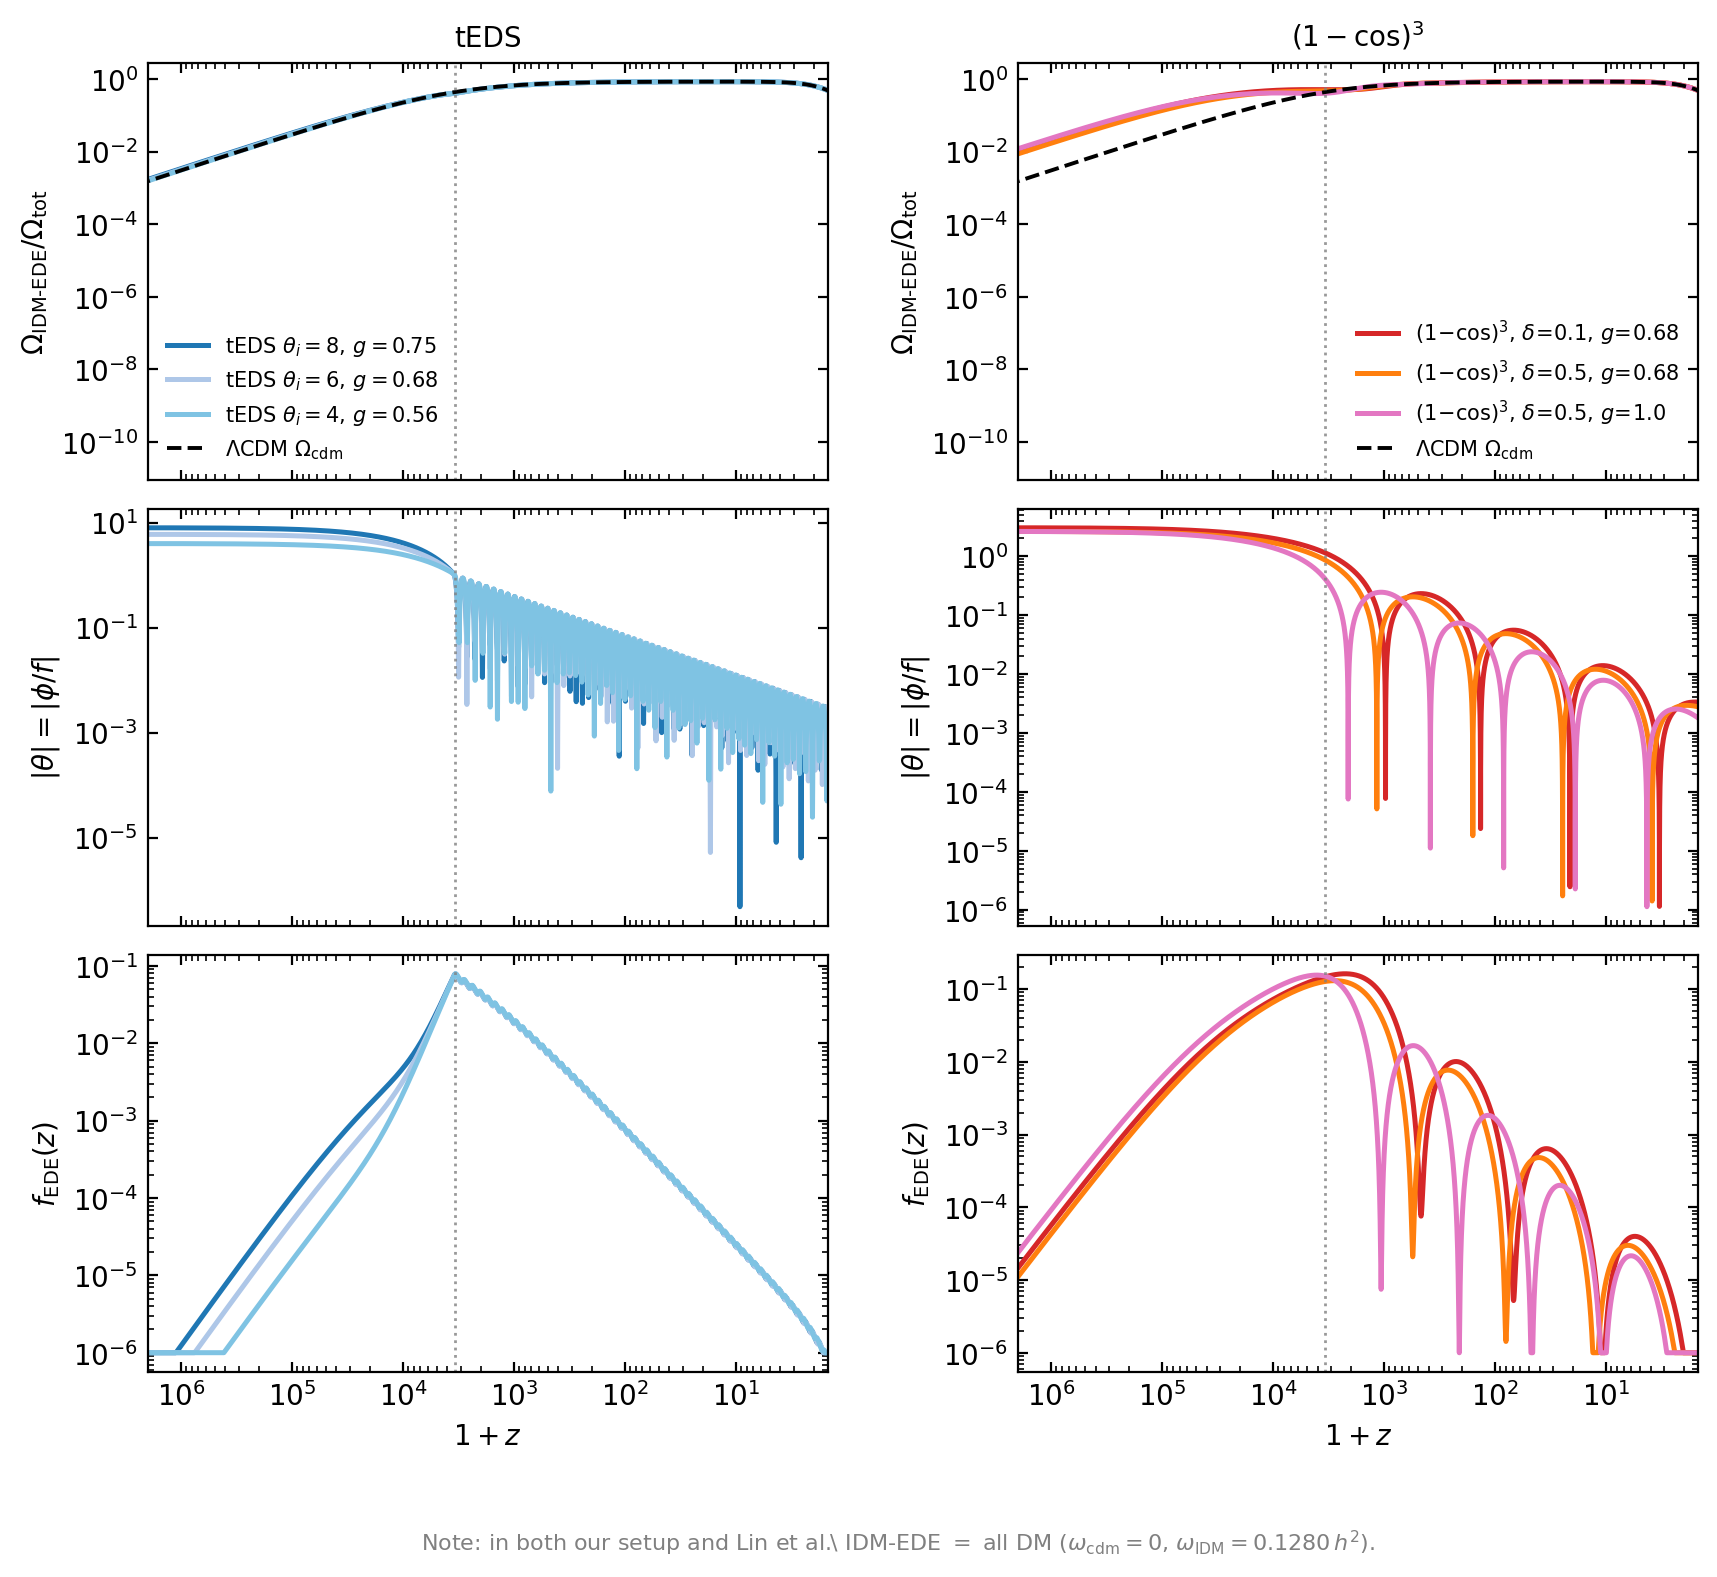
\includegraphics[width=\linewidth]{fig_omega_idm_evolution.png}
    \caption{$\Omega_{\rm IDM\text{-}EDE}/\Omega_{\rm tot}$ (top), $|\theta|(z)$ (middle), and $f_{\rm EDE}(z)$ (bottom) for tEDS (left) and $(1-\cos)^3$ (right), illustrating the normalization bug. The dashed black curve is the $\Lambda$CDM $\Omega_{\rm cdm}/\Omega_{\rm tot}$ reference. Fixing $\Omega_\Lambda=0.685$ produces a spurious CDM component ($\Omega_{\rm cdm}\approx0.21$); after the fix (\texttt{omega\_cdm=0}, CLASS shooting with \texttt{omega\_idm\_ede}), the CDM component vanishes and $\omega_{\rm IDM,0}$ matches the target $0.1280\,h^2$.}
    \label{fig:omega-idm-evol}
\end{figure*}

\section{Comparison of $f_{\rm EDE}$ and $\Omega_{\rm IDM\text{-}EDE}$ between the two models}
\label{app:comparison-figs}

\Cref{fig:omega-compare} directly overlays the IDM-EDE fractional density $\Omega_{\rm IDM\text{-}EDE}/\Omega_{\rm tot}$ and $f_{\rm EDE}$ for the tEDS benchmark ($\theta_i=6$, $g=0.68$) and two $(1-\cos)^3$ cases ($m/H_0=30$, $f=1$, $g=1$ and $g=0.3$). The IDM density tracks CDM at high $z$ and then departs after the mass shift. The EDE bumps peak at comparable redshifts, though the $(1-\cos)^3$ bump is broader and occurs slightly later.

\Cref{fig:selected-histories} shows the natural-parameter $(1-\cos)^3$ scan with $f=1$, $g=1$, and $m/H_0\in\{1,3,10,30,100\}$. The near-degeneracy in peak timing across all $m/H_0$ values is a signature of coupling domination: when the coupling sets the trigger, the timing depends on $g$ and $\rIDM$ rather than on $m$.

\begin{figure}[ht]
    \centering
    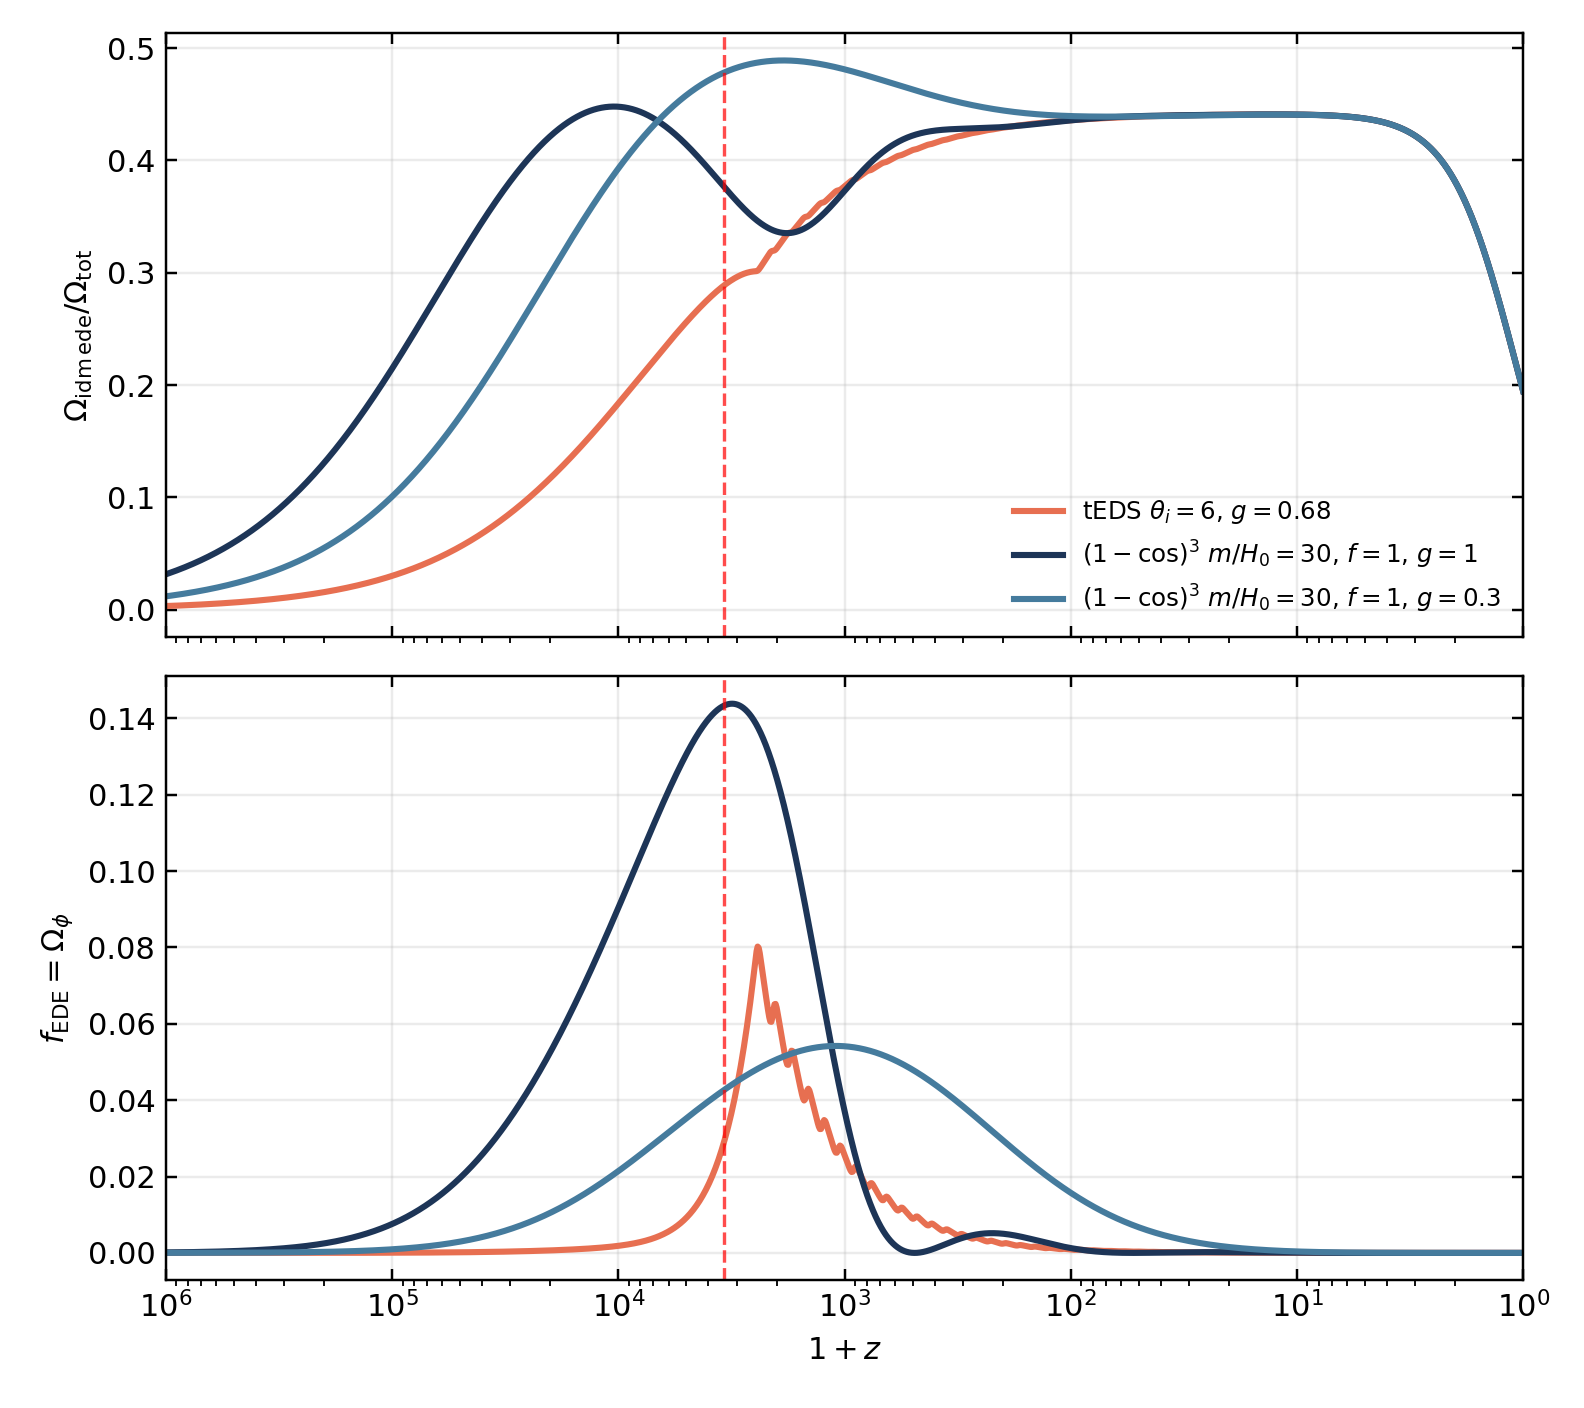
\includegraphics[width=0.90\linewidth]{omega_idm_compare_teds_vs_cos3.png}
    \caption{Direct comparison of $\Omega_{\rm IDM\text{-}EDE}/\Omega_{\rm tot}$ (top) and $f_{\rm EDE}$ (bottom) for the tEDS benchmark ($\theta_i=6$, $g=0.68$) and two $(1-\cos)^3$ benchmarks ($m/H_0=30$, $f=1$, $g\in\{0.3,1\}$). The IDM fraction tracks CDM until the coupling-driven mass shift, while the EDE bumps are qualitatively similar in timing.}
    \label{fig:omega-compare}
\end{figure}

\begin{figure}[ht]
    \centering
    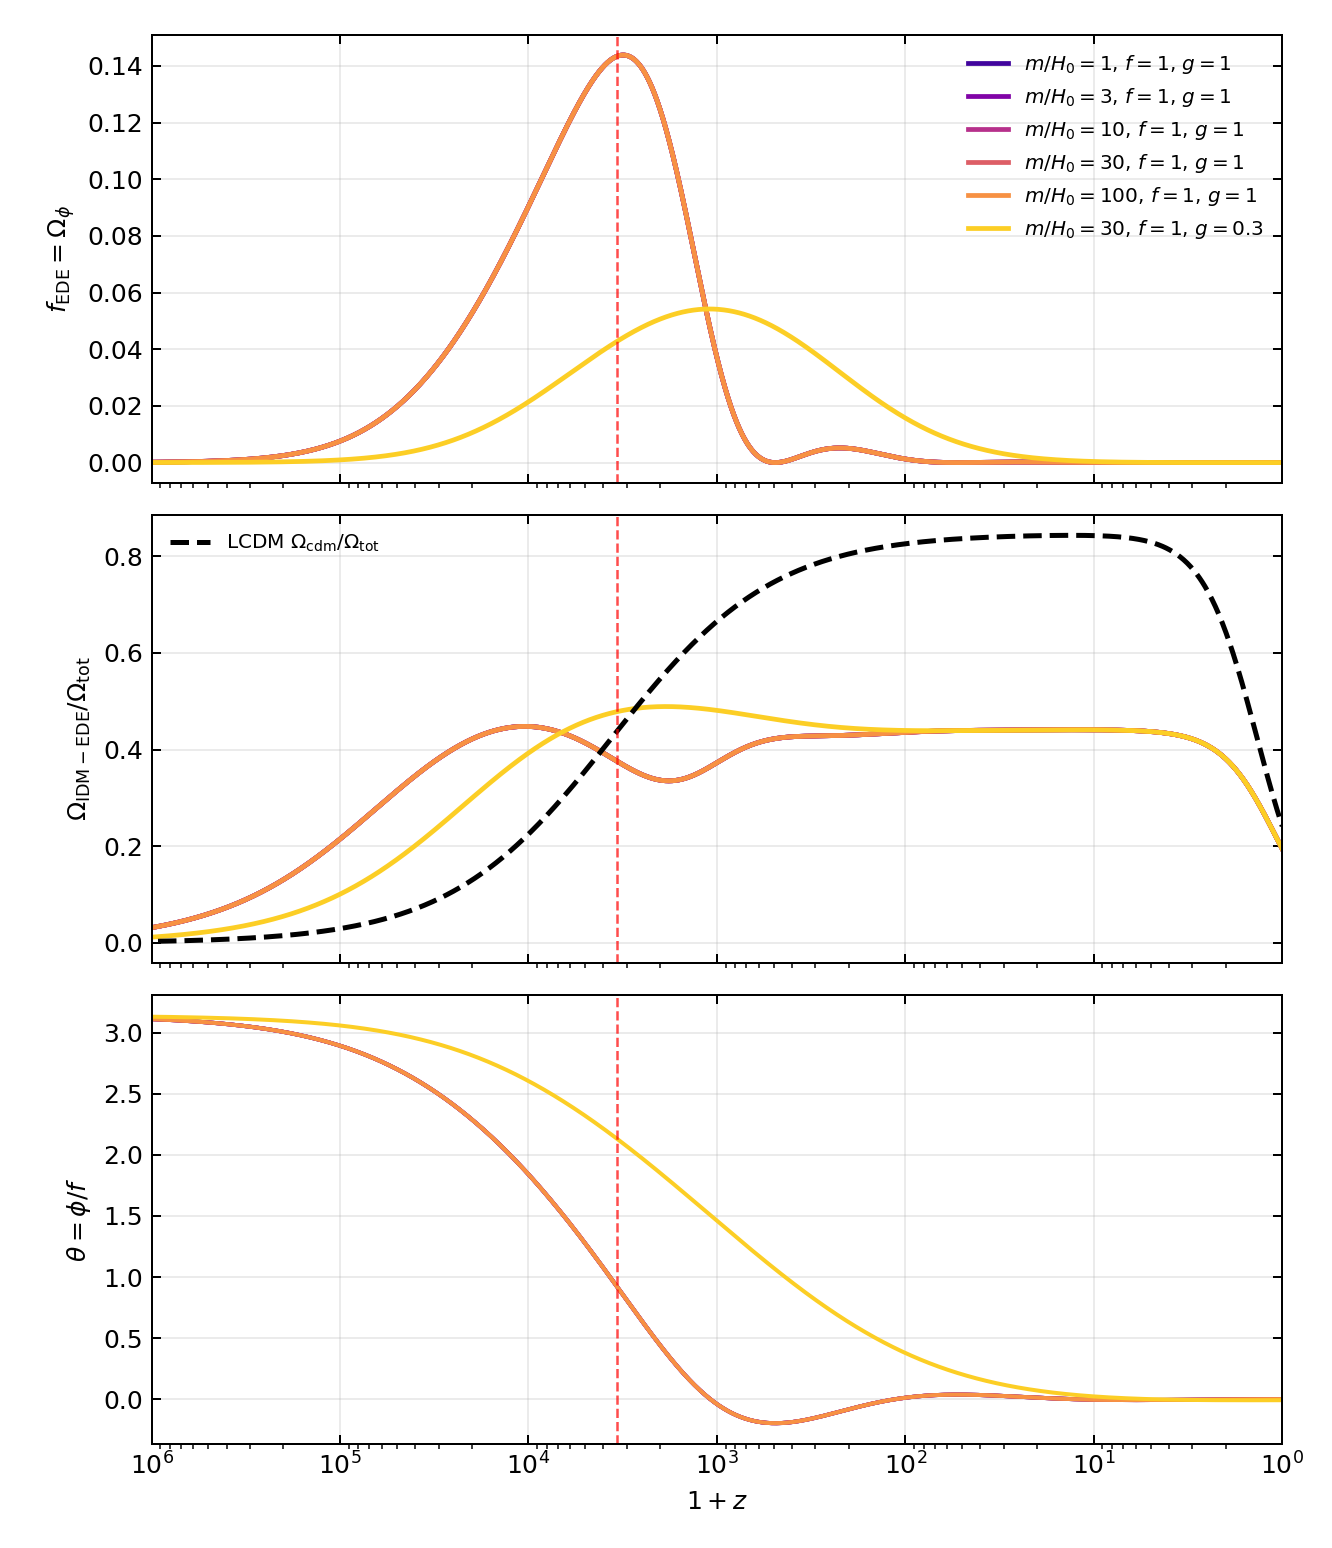
\includegraphics[width=0.90\linewidth]{selected_histories.png}
    \caption{$(1-\cos)^3$ background histories for $f=1$, $g=1$, and $m/H_0\in\{1,3,10,30,100\}$. The near-degeneracy in $f_{\rm EDE}$ peak timing across two decades in $m/H_0$ demonstrates coupling-dominated release: the trigger is set by the IDM dilution rate, not by $m$ alone.}
    \label{fig:selected-histories}
\end{figure}

\section{Debugging history and code changes}
\label{app:debugging}

The results in this paper required several corrections to the AxiCLASS type-1 coupling implementation. We document them here for reproducibility.

\subsection{Corrected type-1 IDM continuity equation}

The original implementation did not include the energy-exchange term due to the time-varying IDM mass. The correct equation is
\begin{equation}
\frac{d\rIDM}{d\ln a} = -3\rIDM + \frac{\phi'}{aH}\,\dlnm\,\rIDM,
\label{eq:rho-idm}
\end{equation}
implemented at \texttt{source/background.c} lines 3386--3388. Without the second term, energy conservation between the scalar field and IDM sectors is violated.

\subsection{Corrected type-1 KG force}

The coupled Klein-Gordon equation must include the full effective slope $V_{,\phi}+3\rIDM\,\dlnm$. An earlier version used only $V_{,\phi}$ in part of the integration, leading to an inconsistency with the IDM continuity equation. The fix is at \texttt{source/background.c} line 3417.

\subsection{Corrected polynomial second derivative}

The perturbation equations require $\partial_\phi^2\ln m$. The correct expression for $m(\phi)=m_0(1+g\phi^2)$ is
\begin{equation}
\partial_\phi^2\ln m = \frac{2g(1-g\phi^2)}{(1+g\phi^2)^2},
\end{equation}
which changes sign at $\phi=1/\sqrt{g}$. An earlier version used a simplified expression that was only valid for $g\phi^2\ll 1$. Fix at \texttt{source/background.c} line 4186.

\subsection{Corrected perturbation-level coupling source}

The perturbation equations were sourced with hard-wired values for $\dlnm$ and $\partial_\phi^2\ln m$ rather than the actual background field values, causing an inconsistency between the background and perturbation sectors for large-field runs. Fix at \texttt{source/perturbations.c} lines 10383--10388 and line 10669.

\subsection{Exponential coupling option}

An exponential coupling $m(\phi)=m_0\,e^{c\phi}$ (constant $\dlnm = c$) was added as \texttt{idm\_ede\_mass\_form = exp} for comparison with the polynomial case. Polynomial coupling saturates at large $\phi$ (since $\dlnm\to 0$ for $g\phi^2\gg1$), whereas exponential coupling provides a constant force per unit IDM density. Implementation: \texttt{source/input.c} lines 3831--3846 and \texttt{source/background.c} lines 4142--4164.

\subsection{Coupled slow-roll initial condition}
\label{app:ic}

Starting from $\dot\phi_{\rm ini}=0$ places the system off the overdamped branch \cref{eq:terminal}, generating an unphysical transient in $\rho_\phi$ before the solution relaxes. \Cref{fig:ic-compare} illustrates this: the old initialization produces a visible spike in the early-time EDE density that disappears when the field relaxes to the terminal branch.

We initialize instead directly on the coupled terminal branch,
\begin{equation}
\phi'_{\rm ini} = -\frac{a}{2H}\!\left(V_{,\phi}+3\rIDM\,\dlnm\right)\!\Big|_{\rm ini}.
\label{eq:ic}
\end{equation}
The factor of $2$ (vs.\ the $3H$ in the cosmic-time slow-roll formula) comes from the $-2\phi'$ damping term in the $\ln a$-form KG equation (see \cref{app:bg-eqs}); setting $d\phi'/d\ln a=0$ gives exactly \cref{eq:ic}. The late-time evolution is unchanged. Implementation: flag \texttt{coupled\_scf\_slowroll\_ic}, enabled by default for type-1 runs; \texttt{source/background.c} lines 2966--2979 and \texttt{include/background.h} line 220.

\begin{figure}[ht]
    \centering
    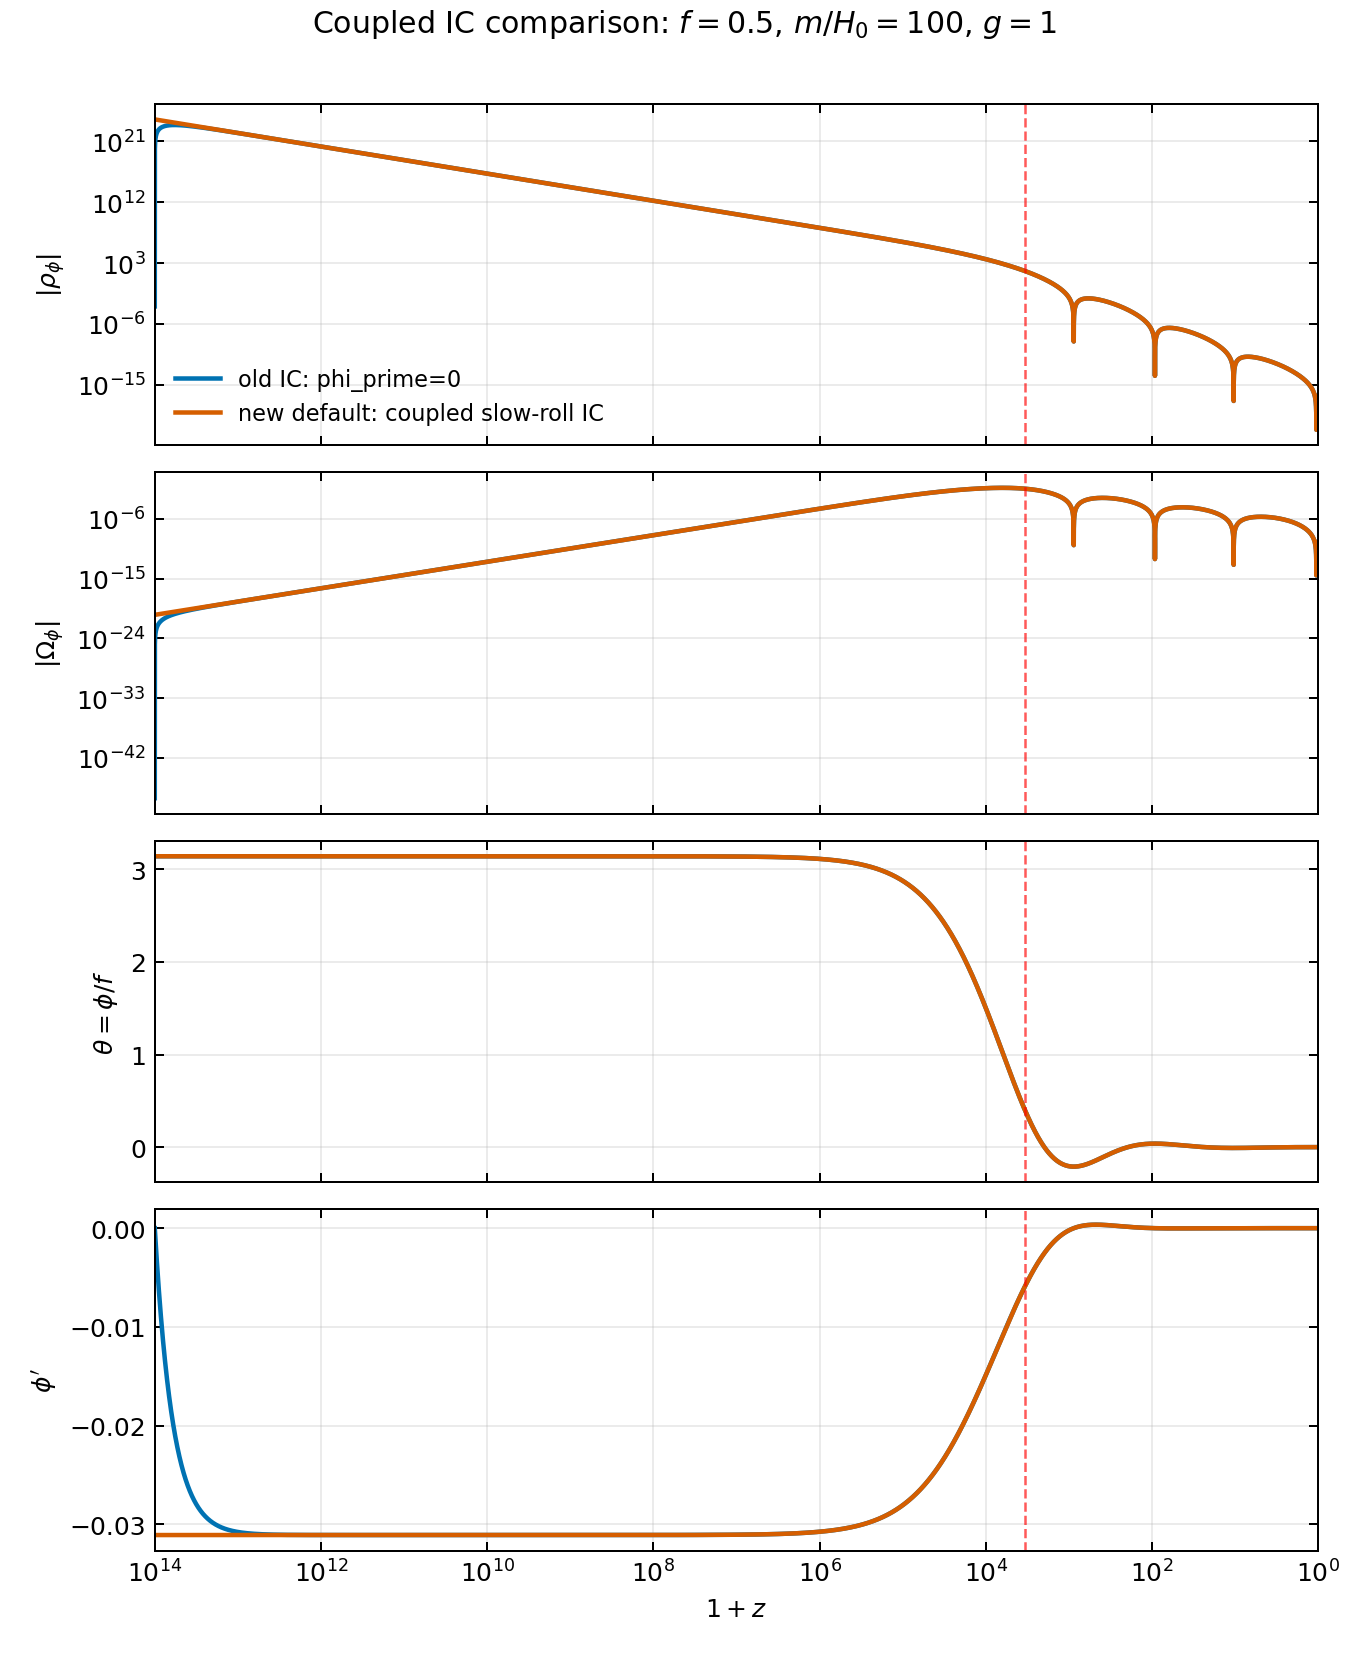
\includegraphics[width=0.92\linewidth]{coupled_ic_comparison_m100_f0p5_g1.png}
    \caption{Effect of the initial condition for $(f,\,m/H_0,\,g)=(0.5,\,100,\,1)$. The old initialization with $\phi'_{\rm ini}=0$ produces a transient spike in the EDE density at early times (dashed). The corrected coupled slow-roll IC starts on the overdamped branch, removing the artifact without changing the late-time history (solid).}
    \label{fig:ic-compare}
\end{figure}

\subsection{Background equations}
\label{app:bg-eqs}

The implemented $\ln a$-form equations are:
\begin{align}
\frac{d\phi}{d\ln a} &= \frac{\phi'}{aH},\\
\frac{d\phi'}{d\ln a} &= -2\phi' - \frac{a}{H}\!\left(V_{,\phi}+3\rIDM\,\dlnm\right),\\
\frac{d\rIDM}{d\ln a} &= -3\rIDM + \frac{\phi'}{aH}\,\dlnm\,\rIDM.
\end{align}

\subsection{Polynomial coupling derivatives}

For $m_{\rm IDM}(\phi)=m_0(1+g\phi^2)$:
\begin{equation}
\dlnm = \frac{2g\phi}{1+g\phi^2},\qquad
\partial_\phi^2\ln m = \frac{2g(1-g\phi^2)}{(1+g\phi^2)^2}.
\end{equation}
Both expressions are evaluated at the current background field value at each time step, in both the background (\texttt{source/background.c} line 4186) and perturbation (\texttt{source/perturbations.c} lines 10383--10388) equations.

\subsection{Corrected $V_0$ unit conversion}

The tEDS potential normalization $V_0$ is specified in CLASS units of $\mpl^2/\text{Mpc}^2$. The conversion from physical units (eV$^4$) is
\begin{equation}
V_0^{\rm CLASS} = V_0^{\rm eV^4} \times \left(\frac{1\,\text{Mpc}^{-1}}{m_{\rm Pl}}\right)^{-2} = V_0^{\rm eV^4} \times \left(\frac{1.56\times10^{29}\,\text{eV}}{2.435\times10^{27}\,\text{eV}}\right)^2 \approx V_0^{\rm eV^4} \times 4104.
\end{equation}
An earlier version of the analysis scripts used an extra factor of $1/3$ in this conversion, motivated by the fact that \texttt{background.c} line~514 computes $\tilde{\rho}_{\rm scf} = (K+V)/3$. This was incorrect: the factor of $1/3$ is already internal to CLASS and should not appear in the conversion of $V_0$. With the spurious factor the stored $V_0$ was three times too small, giving $f_{\rm EDE}\approx 4\%$ instead of the correct $\approx 8\%$ for $V_0=0.08\,{\rm eV}^4$. The fix: remove the $/3$ from \texttt{EV4\_TO\_CLASS} and use $V_0^{\rm eV^4}=0.10$ (matching Ref.~\cite{Lin:2022teds} Fig.~2 peak $f_{\rm EDE}\approx10\%$).

\subsection{Fixed CLASS internal shooting for \texttt{omega\_idm\_ede}}

The original \texttt{target\_namestrings}/\texttt{unknown\_namestrings} arrays in \texttt{source/input.c} had the IDM-EDE target and unknown roles reversed: \texttt{omega\_ini\_idm\_ede} was listed as the target and \texttt{omega\_idm\_ede} as the unknown, causing the shooter to solve a fixed-point problem that ignored the user's desired today density.

The fix adds two new enum values \texttt{Omega\_idm\_ede\_today}/\texttt{omega\_idm\_ede\_today} (indices 14--15) to \texttt{include/input.h} (updating \texttt{\_NUM\_TARGETS\_} from 14 to 16) and the corresponding entries in the three arrays (\texttt{target\_namestrings}, \texttt{unknown\_namestrings}, \texttt{target\_cs}) in \texttt{source/input.c}. The initial guess and bracket-search Jacobian are set in \texttt{input\_get\_guess} (new \texttt{case Omega\_idm\_ede\_today}). The shooting output function already computes the correct residual $\Omega_{\rm IDM,0}^{\rm target} - \rho_{\rm IDM,0}/H_0^2$, which is shared with the output cases for the existing (swapped) targets. The bracket-search Jacobian sign is $-0.5$ (negative): increasing $\omega_{\rm ini}$ gives a larger today density, making the residual more negative.

\subsection{Input parser: mass-form switch}

The parser accepts \texttt{idm\_ede\_mass\_form = poly} (polynomial), \texttt{exp} (exponential), \texttt{phantom}/\texttt{andriot}/\texttt{am} (phantom-sector forms). The type-1 coupling path parses the mass form and defaults at \texttt{source/input.c} lines 3821--3846 and 7707.

\begin{figure*}[ht]
    \centering
    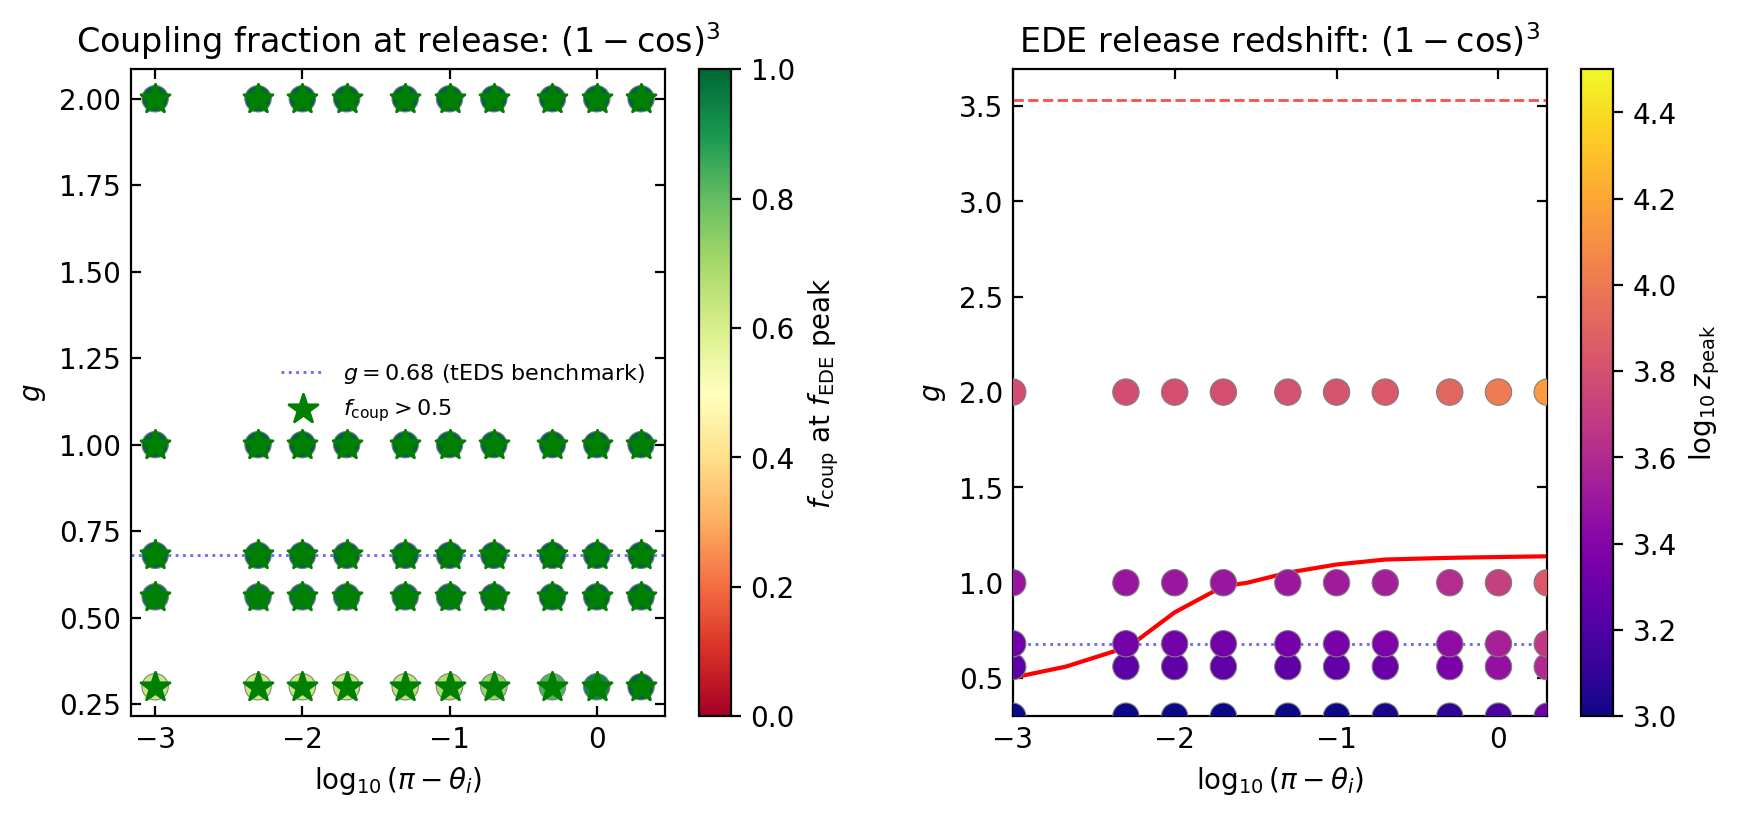
\includegraphics[width=\linewidth]{fig1_zpeak_vs_delta.png}
    \caption{Left: coupling fraction $\fcoup$ at the $f_{\rm EDE}$ peak for $(1-\cos)^3$ in the $(\log_{10}\delta,\,g)$ plane ($\delta\equiv\pi-\theta_i$). Green stars mark coupling-dominated cases ($\fcoup>0.5$). The dashed blue line is the tEDS benchmark $g=0.68$. Right: release redshift $\log_{10}z_{\rm peak}$ in the same plane; the red dashed line marks $z_{\rm eq}$, and the red contour traces $z_{\rm peak}=z_{\rm eq}$. Nearly all tested cases are coupling-dominated. The release redshift increases with $g$ (stronger coupling → earlier trigger) and is nearly independent of $\delta$ for $g\gtrsim 0.56$.}
    \label{fig:zpeak}
\end{figure*}

\begin{figure*}[ht]
    \centering
    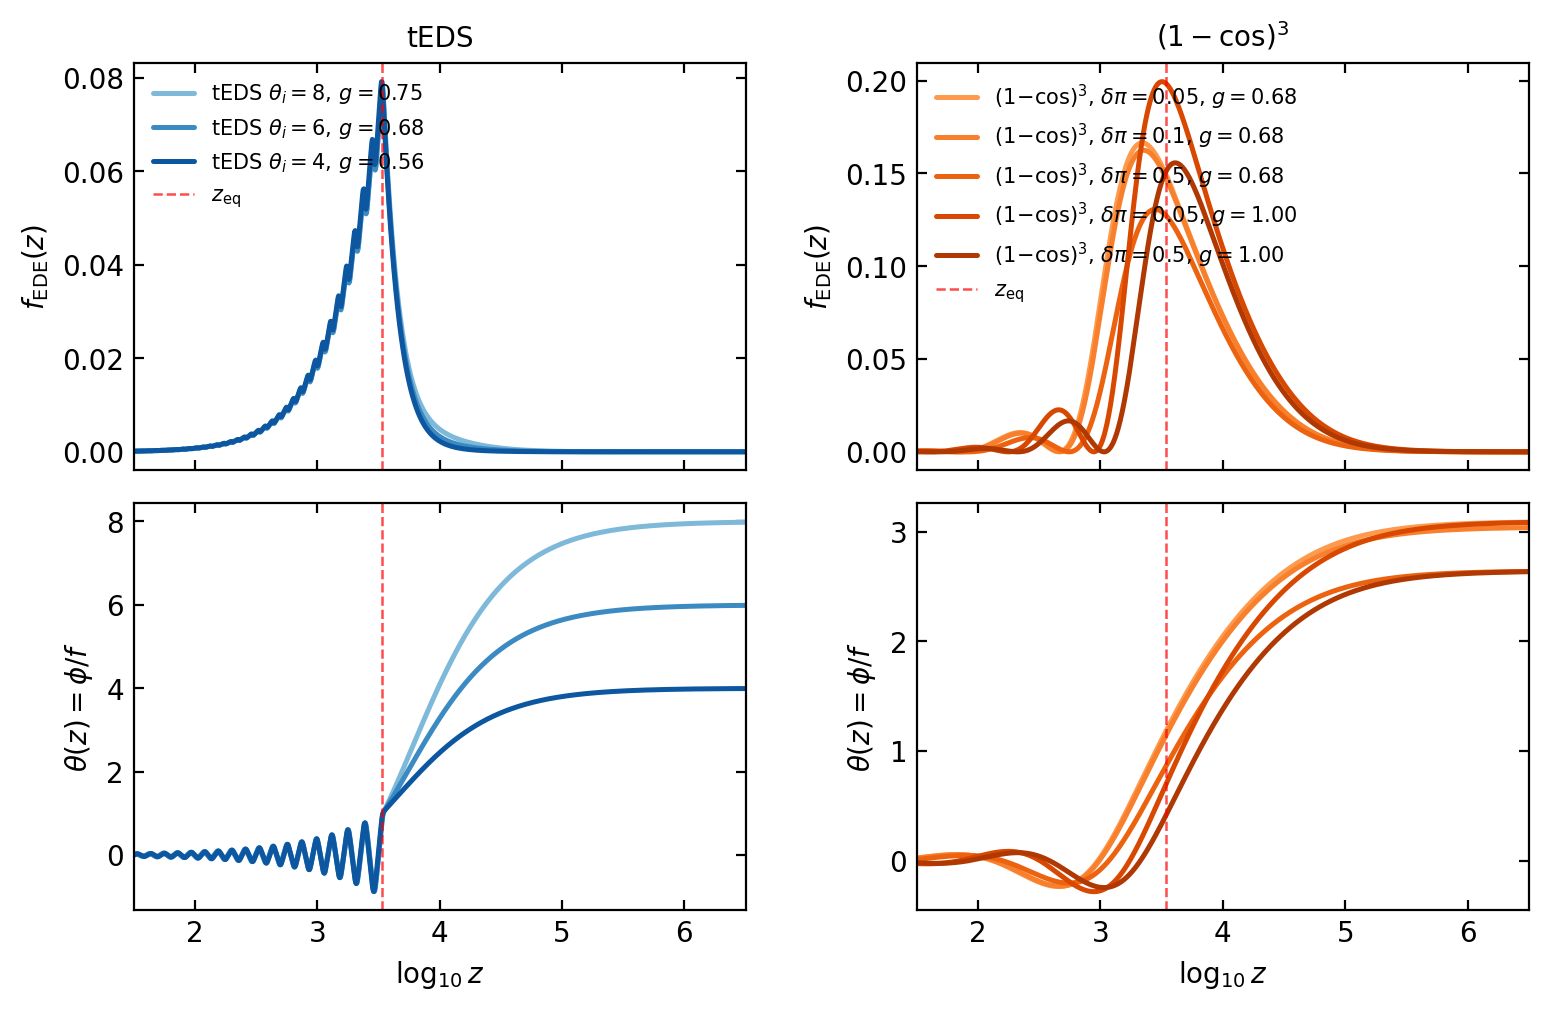
\includegraphics[width=\linewidth]{fig2_histories.png}
    \caption{EDE histories for tEDS (left column) and $(1-\cos)^3$ (right column). Top: $f_{\rm EDE}(z)$. Bottom: normalized field $\theta(z)=\phi/f$. The dashed vertical line marks $z_{\rm eq}$. In tEDS the field rolls off the plateau and rapidly decays to $\theta\to 0$, producing a sharp $f_{\rm EDE}$ bump. In $(1-\cos)^3$ the field drifts slowly away from the hilltop, producing a broader bump.}
    \label{fig:histories}
\end{figure*}

\begin{figure}[ht]
    \centering
    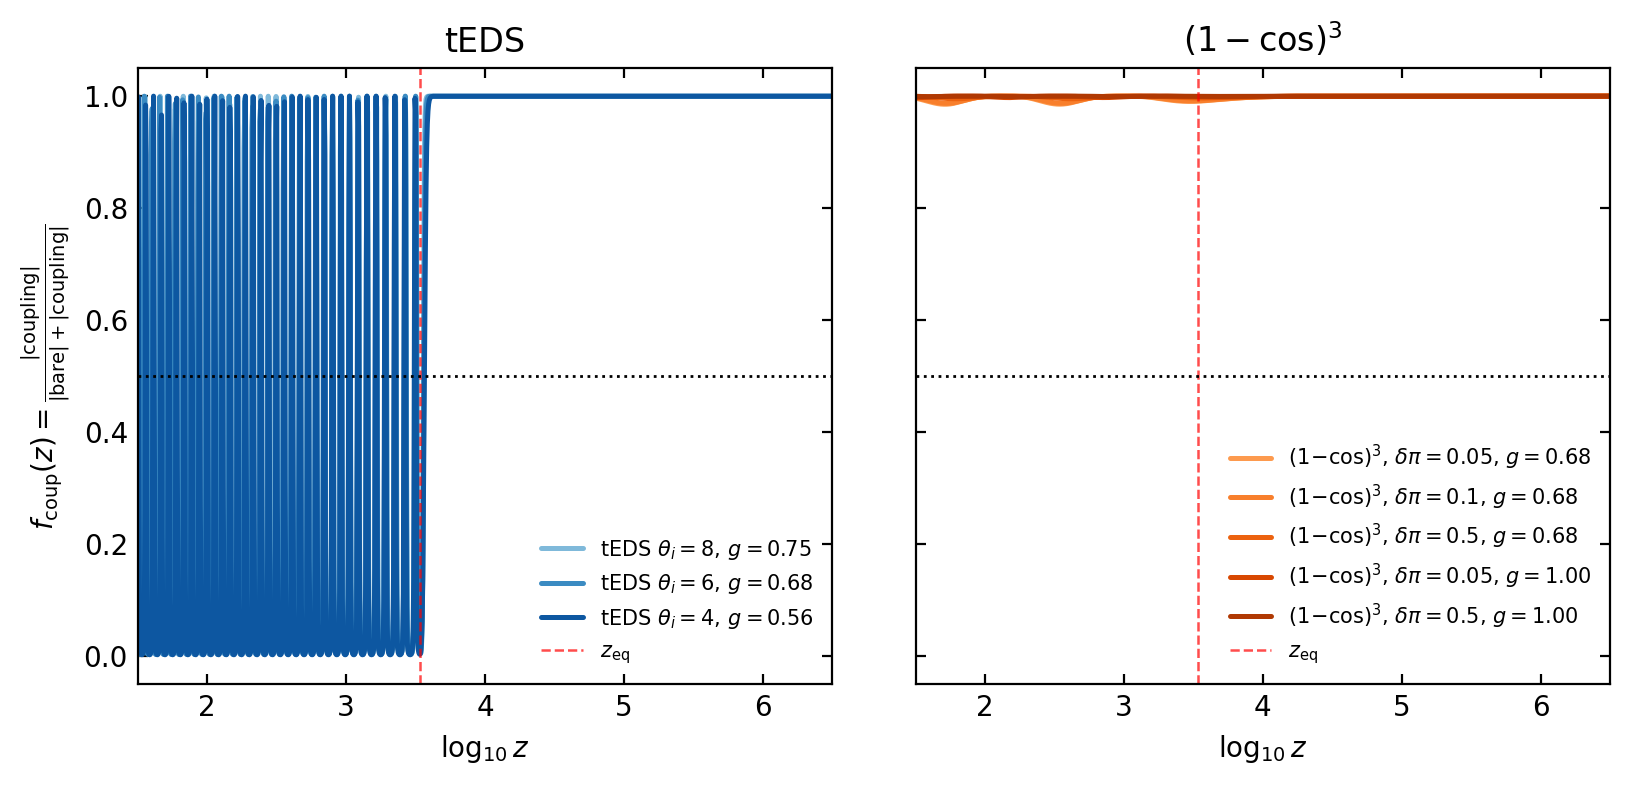
\includegraphics[width=0.96\linewidth]{fig3_trigger_coupling.png}
    \caption{Coupling fraction $\fcoup(z)$ as a function of redshift. Left: tEDS benchmarks. Right: $(1-\cos)^3$ with $g=0.68$ and $\delta\in\{0.05,\,0.1,\,0.5\}$ and $g\in\{0.68,1\}$. In both potentials $\fcoup\approx 1$ at $z>z_{\rm eq}$, confirming coupling-dominated release. For tEDS, after rolling off the plateau the field oscillates rapidly around $\phi=0$, causing fast oscillations in $\fcoup$ (the ratio $|{\rm coupling}|/|V'|$ alternates sign as the field passes through zero). In $(1-\cos)^3$ the field drifts slowly away from the hilltop and $\fcoup$ remains $\approx 1$ throughout since the bare slope is always negligible near $\theta=\pi$.}
    \label{fig:trigger-coupling}
\end{figure}

\begin{figure}[ht]
    \centering
    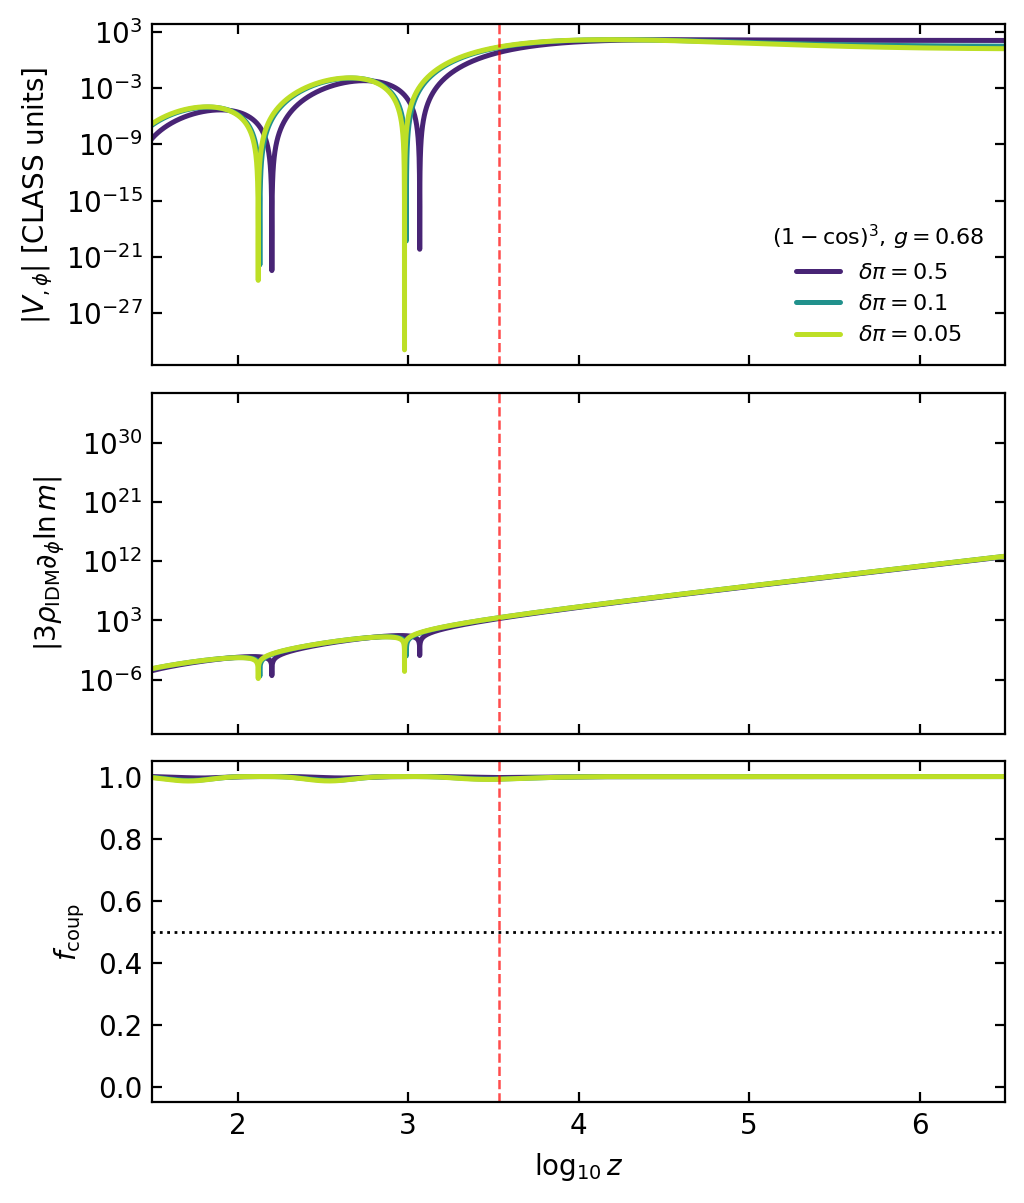
\includegraphics[width=0.72\linewidth]{fig4_force_budget.png}
    \caption{Force budget for $(1-\cos)^3$ at $g=0.68$ and $\delta\in\{2,\,0.5,\,0.1,\,0.01\}$. Top: bare slope $|V_{,\phi}|$. Middle: coupling term $|3\rIDM\dlnm|$. Bottom: coupling fraction $\fcoup(z)$. The coupling dominates ($\fcoup\approx 1$) from high redshift until well past the EDE peak for all $\delta$ values. The bare slope is orders of magnitude smaller than the coupling term at $z\gtrsim 10^4$ regardless of $\delta$.}
    \label{fig:force-budget}
\end{figure}

\begin{thebibliography}{99}
\bibitem{Poulin:2018cxd}
V.~Poulin, T.~L.~Smith, T.~Karwal, and M.~Kamionkowski,
``Phasing in Planck Data Post Recombination and the Hubble Tension,''
\href{https://arxiv.org/abs/1811.04083}{arXiv:1811.04083}.

\bibitem{Smith:2019ihp}
T.~L.~Smith, V.~Poulin, and M.~A.~Amin,
``Oscillating scalar fields and the Hubble tension: a resolution with novel signatures,''
\href{https://arxiv.org/abs/1908.06995}{arXiv:1908.06995}.

\bibitem{McDonough:2021}
E.~McDonough, M.-X.~Lin, J.~C.~Hill, W.~Hu, and S.~Zhou,
``The Early Dark Sector, the Hubble Tension, and the Swampland,''
\href{https://arxiv.org/abs/2112.09128}{arXiv:2112.09128}.

\bibitem{Lin:2022teds}
M.-X.~Lin, E.~McDonough, J.~C.~Hill, and W.~Hu,
``A Dark Matter Trigger for Early Dark Energy Coincidence,''
\href{https://arxiv.org/abs/2212.08098}{arXiv:2212.08098}.
\end{thebibliography}

\end{document}
